\documentclass[a4paper,12pt]{article}
\usepackage[utf8]{inputenc}
\usepackage[T1]{fontenc}
\usepackage[spanish]{babel}
\usepackage{csquotes}
\usepackage{anysize}
\usepackage{graphicx}
\marginsize{25mm}{25mm}{25mm}{25mm}

\title{Time horizons in rats foraging for food in temporally separated patches}
\author{William Timberlake \and Donald J. Gawley \and Gary A. Lucas}
\date{1987}

\begin{document}
{\scshape\bfseries \maketitle}

El forrajeo óptimo se ocupa de la selección de fuentes de comida para explotar a través del tiempo. Un problema clásico es cuánto tiempo un animal debe permanecer por parche antes de pasar a otro (``{\itshape giving-up time}''). Según el teorema de valor marginal de Charnov los forrajeadores deberían abandonar un parche cuando la tasa de encuentro de presas cae por debajo de la tasa promedio de parches alternativos. Hay evidencia razonable que apoya esta predicción, lo que indica que los animales se comportan como consumidores racionales.

Pero es necesario conocer el período de tiempo en el que los animales comparan fuentes de comida alternativas. Esta ventana de integración ha sido referida como el {\itshape horizonte temporal} de un animal, y no se ha estudiado dado que usualmente los parches están disponibles de forma simultánea, con lo que el tiempo depende solo de la separación o el programa.

En la naturaleza los tiempos de viaje pueden ser largos para algunas especies, y ciertas fuentes de comida están más accesibles (son menos costosas) en momentos particulares del día. Por lo tanto los animales deben organizar su forrajeo en el tiempo también.

Timberlake encontró que las ratas no muestran consumo ``racional'' cuando el acceso a un parche que se depleta (simulado por razón progresiva) precede el acceso a un parche más rico por una hora o más.

Una visión de optimalidad que solo incluye la ingesta y costo de respuesta actuales no tiene en cuenta la distancia temporal.

Parece se que los organismos tienden a descontar las respuestas futuras como una función incremental de la distancia temporal. Esto parece adaptativo en ambientes impredecible o peligrosos en los que una presa ya capturada vale más que otra potencial pero incierta. Así, debería haber un efecto de supresión de la comida futura sobre el forrajeo actual que declina con la distancia temporal.

Pero en el estudio de Timberlake no se encontró supresión incluso con una demora de solo una hora: en todas las condiciones las ratas se forrajeaban como si no existiese comida futura. Esto sugiere que el horizonte temporal para que las ratas comparen fuentes alternativas de comida es de menos de una hora.

El propósito de este estudio es determinar el intervalo de tiempo en el que una fuente de comida más rica disminuirá el forrajeo de un parche que se agota. Se emplearán dos parches físicamente separados disponibles de forma continua para el animal. Los parches consistían en dos áreas con una barra y acceso aun comedero. Un parche estaba siempre disponible con un programa de razón progresiva (PR). El segundo tenía un programa de reforzamiento continuo (CRF) y se hacía disponible tras una demora fija desde el inicio de la sesión (entre 4 y 120 minutos).

Otro propósito fue determinar si los resultados negativos de Timberlake se debieron a un artefacto: que los sujetos estaban obligados a permanecer en un parche que se agota durante una hora, cuando en la naturaleza podrían abandonarlo en cualquier momento y evitar el contacto con las claves relacionadas con comida que elicitan las respuestas. Para ello se comparó la conducta de ratas que podían abandonar el parche que se agota con ratas que no podían.

El tercer propósito de la investigación fue investigar la posibilidad de que el horizonte temporal no sea un fenómeno unitario. Timberlake no anticipó la posibilidad de que las ratas pueden anticipar la disponibilidad de la comida futura sin disminuir el forrajeo actual. Este estudio midió tanto el decremento en el forrajeo actual como la anticipación de la comida futura. Lo primero fue medido comparando la ingesta en el PR bajo demoras menores a la comida futura con la ingesta cuando la comida futura tenía demoras de 2 horas. La anticipación fue medida según el tiempo pasado y el número de presiones de las barras en el parche CRF antes de que la comida estuviera disponible ahí.

{\scshape\bfseries Method}

La caja operante se presenta en la figura 1. Los dos parches se encontraban separados por una pieza en forma de T de metal que formaba un túnel en la parte frontal de la caja.

\begin{figure}[hb]
	\begin{center}
		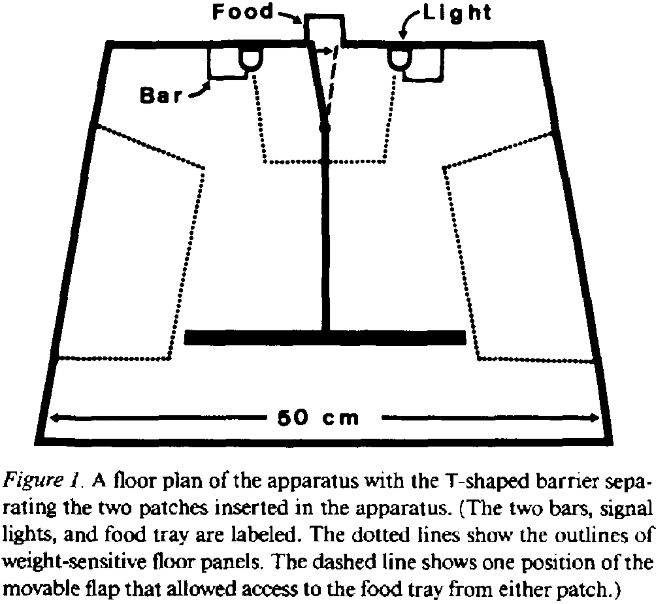
\includegraphics[scale=0.5]{Timberlake1987(1).png}
	\end{center}
\end{figure}

El régimen de privación de comida no fue mantenido durante el experimento, sino solamente en el inicio durante la adquisición de la presión de las barras, sino que, adicional a la comida obtenida en el parche PR, se proveían 32 minutos adicionales en el parche CRF.

Los animales tenían acceso continuo a ambos parches en todo momento. Para el grupo de barrera la presencia de la T los obligaba a viajar 80 cm para pasar de una barra a la otra. Cada sesión comenzaba con la extensión de ambas barras, pero solo la PR estaba operativa (indicado por su luz encendida). La palanca CRF se hacía operativa tras un tiempo fijo y se encendía su luz. En la condición con barrera las ratas debían abandonar el parche FR para ver la luz; pero en la condición si barrera, no. Esta diferencia no pareció afectar las respuestas.

Las demoras de CRF fueron de 32, 16, 8, 4, 16, 32, 64, 120 minutos en ese orden. Todas las demoras estuvieron vigentes por 18 a 24 sesiones. El cambio de una condición a otra era decidido por inspección visual. 

En las demoras de 64 minutos hacia abajo los sujetos permanecieron en el aparato. Para la demora de 120 minutos, permanecieron en él solo durante los primeros 64, luego de lo cuál fueron regresados a sus caja habitación durante aproximadamente una hora, para luego ser regresados al aparato para concluir sus 32 minutos de CRF. Toda la comida fue recibida dentro del aparato sin restricciones.

Se registraba una entrada a un parche cuando el animal presionaba el panel lateral sensible al peso o presionaba la barra correspondiente. El tiempo pasado en un parche se acumulaba en tanto el animal siguiera respondiendo, presionando el panel lateral, o entrando en el comedero con una separación máxima de 15 segundos.

Los análisis estadísticos se hicieron con base en el último bloque de seis sesiones para cada condición.

{\scshape\bfseries Results}

La presencia de la barrera no afectó la ingesta total de pellets en el parche PR, por lo que se combinaron los datos de ambos grupos.

Las ratas consumieron menos comida durante las condiciones de 4, 8, y 16 minutos de demora que en los mismos intervalos de tiempo en la condición de referencia (2 horas), pero las condiciones de 32 y 64 minutos no difirieron significativamente de la referencia. Además la ingesta en las condiciones de 4 y 8 era menor que la ingesta en las demás condiciones, y que ésta no difirió entre ninguna de las demás.

Se presume que la condición de referencia indica cómo se desempeñan los animales cuando se espera que la comida futura no tenga ningún efecto en las respuestas actuales.

El tamaño del efecto supresor de la ingesta estaba inversamente relacionado con la distancia temporal a la comida.

Tanto la presión anticipada de la barra como el tiempo pasado en el parche CRF mostraron una clara anticipación de la disponibilidad de comida en todos los intervalos, con la posible excepción de la condición de 64 minutos.

La única diferencia notable entre los grupos de barrera y no barrera fue el tiempo promedio de visita durante cada condición. Se realizó un análisis de varianza para comparar el tiempo promedio de visita en el último bin de cada condición de demora para ambos grupos. El análisis reveló un efecto significativo de la interacción entre la barrera y la demora.

Una prueba de efectos principales mostró que el tiempo de visita promedio en el parche CRF en el último bin fue significativamente mayor en el grupo de barrera que en el de no barrera para las demoras de 8, 16 y 32 minutos, pero no para las de 4 y 64. Esto apoya a la predicción de la teoría de forrajeo óptimo que indica que cuanto mayor sea la distancia entre parches, mayor será el tiempo de visita, y también apoya el hallazgo anterior de que la anticipación al acceso a la comida en el parche CRF disminuyó con demoras mayores.

{\scshape\bfseries Discussion}

Las ratas fallaron en disminuir su forrajeo actual en un parche que se agota cuando un parche futuro más rico estaba demorado por más de 16 minutos. Dentro de esta ventana de 16 minutos la supresión estaba inversamente relacionada con el período de demora, pero el grado de supresión fue pequeño comparado con lo que se requería para que las ratas maximizaran su ingesta por costo de respuesta.

Esto apoya el reporte de Timberlake que indica que las ratas no mostraron el efecto de supresión por la comida futura en las respuestas actuales cuando los parches estaban separados por una hora o más.

Se había sugerido que quizá sus ratas no mostraron la supresión dado que no podían abandonar el parche y pasar a otro, pero este experimento no apoyó esa hipótesis dado que la ingesta de animales en parches claramente separados no fue distinta de la de animales incapaces de alejarse físicamente de las claves asociadas con el parche que se agota (el grupo sin barrera).

Otros estudios han reportado rangos temporales similares para la supresión. Un experimento estudió la habilidad de chimpancés para cambiar óptimamente entre un programa PR y uno de razón fija (FR) que reiniciaba el valor del PR a 1. Se encontró que los simios se aproximaban al mínimo costo de respuesta por recompensa al cambiar al FR bastante antes de que el valor de PR igualara al de FR. El tiempo en que los animales parecían medir la recompensa de los programas combinados era de 15 minutos.

En general se ha encontrado que la supresión funciona solamente en tiempo muy breves, aunque hay un experimento en que se ha encontrado supresión de consumo de sacarina cuando se da acceso a una solución preferida 30 minutos después.

En breve, los estudios apoyan la idea de que los animales tienen un período breve en el cual se comportan de forma efectiva con respecto a alternativas de alimentación temporalmente separadas. Y aun en esas ventanas la alocación de conducta no es óptima en términos de comida por costo de respuesta. Los animales pagan un precio muy alto por la comida como para estar actuando como consumidores racionales.

Que el forrajeo costoso disminuya poco puede tener sentido en una visión de causas finales. Una tendencia a esperar por la comida futura sería eliminada por la selección natural dado que la comida futura es más incierta que la comida actual. Especies en ambientes más impredecibles y con más depredadores deberían tener este sesgo a favor de la comida presente en mayor medida.

{\scshape Interdependence of suppression and anticipation}

Estos datos permiten separar los efectos de anticipación y de supresión de la comida futura. Esto puede explicarse con la presencia de dos distintos procesos u horizontes temporales. Pero los datos son compatibles con el argumento de que ambos efectos resultaron de un solo proceso de anticipación. La supresión sucedió solo cuando las actividades anticipatorias compitieron temporalmente con el forrajeo actual. Sin embargo, no está claro si la competencia por sí misma puede explicar el tamaño del efecto de supresión, por lo que no se puede descartar la hipótesis de la presencia de dos procesos distintos.

{\scshape Time horizons and optimal foraging theory}

Hay considerable evidencia sobre las estrategias óptimas de los animales al explotar fuentes alternativas de comida, pero toda suele ser con fuentes concurrentes y en ambientes más naturales. Estos datos son difíciles de reconciliar con estos hallazgos.

Es posible que las simulaciones de laboratorio dejen de lado aspectos de la situación de forrajeo críticos para la conducta óptima. Por otro lado, es posible que la manejabilidad matemática de la teoría de forrajeo óptimo nos haya llevado a la presunción errónea de que los animales usan un simple algoritmo para comparar los recursos alternativos sin importar su distribución temporal. Parece más probable que la conducta óptima sea resultado de un buen ajuste entre el ambiente y un conjunto complejo de mecanismos de forrajeo que van de la integración a corto plazo a la anticipación a largo plazo.

Si una animal anticipa bien la comida, entonces mecanismos locales pueden explicar bien su conducta.

Quizá no haya un solo horizonte temporal o proceso de timing. Los horizontes deberían variar con los mecanismos usados. Podían variar con las estaciones, días, horas o minutos. Los horizontes de anticipación podrían ser considerablemente más largos que los de supresión. También el costo de las respuestas y el valor incentivo podrían tener un efecto.

Estos resultados y especulaciones sugieren que la conducta de forrajeo tiene determinantes más complejos que los que se asumen por algoritmos generales de optimalidad que no consideran cuidadosamente la escala temporal.

\end{document}
